%\documentclass{article}
%\usepackage[pdftex,active,tightpage]{preview}
%\usepackage{tikz}
%\usetikzlibrary{arrows,shapes,backgrounds}
%\begin{document}
%\begin{preview}
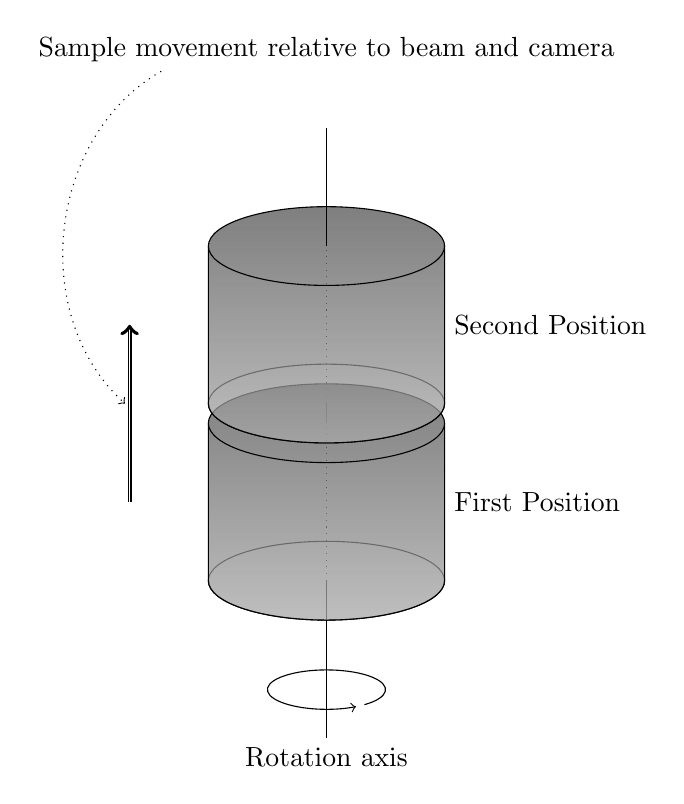
\begin{tikzpicture}%[ultra thick,scale=1]%,show background grid]
	%draw axes
		%\draw[ultra thick] (-10,0) -- (10,0);
		%\draw[ultra thick] (0,-10) -- (0,10);
		%\draw[ultra thick] (0,0) circle (.125);
	% rotation axis
		\draw[->] (0,-2) ++ (-50:.75) arc (-50:300:.75 and .25);
		\draw (0,-3) node [below] {Rotation axis} -- ++(0,2);
		\draw[dotted] (0,-1) -- ++(0,2);
		\draw (0,1) -- ++(0,0.25);
		\draw[dotted] (0,1.25) -- ++(0,2);
	% position 1
		\draw (0,-1) circle (1.5 and .5);
		\fill[shade,semitransparent] (-1.5,-1) arc (-180:0:1.5 and .5) -- ++(0,2) arc (0:180:1.5 and .5) -- cycle;
		\draw (-1.5,-1) arc (-180:0:1.5 and .5) -- ++(0,2) arc (0:180:1.5 and .5) -- cycle;		
		\draw (-1.5,1) arc (-180:0:1.5 and .5);
		\draw (1.5,0) node [right] {First Position};
	% position 2
		\draw (0,1.25) circle (1.5 and .5);
		\fill[shade,semitransparent] (-1.5,1.25) arc (-180:0:1.5 and .5) -- ++(0,2) arc (0:180:1.5 and .5) -- cycle;
		\draw (-1.5,1.25) arc (-180:0:1.5 and .5) -- ++(0,2) arc (0:180:1.5 and .5) -- cycle;		
		\draw (-1.5,3.25) arc (-180:0:1.5 and .5);
		\draw (1.5,2.25) node [right] {Second Position};
	% rotation axis on top
		\draw (0,3.25) -- ++(0,1.5);									
	% sample movement
		\draw[double,->] (-2.5,0) -- (-2.5,2.25);% node [text width=10cm,midway,left] {Sample movement relative to beam and camera};	
		% sample movement
		\node (movefrom) at (0,5.75) {Sample movement relative to beam and camera};
		\node (moveto) at (-2.5,1.125) {};
		\draw [->,dotted] (movefrom) to [bend right=54] (moveto);
\end{tikzpicture}
%\end{preview}
%\end{document}